\documentclass[a4paper,11pt]{article}

\usepackage[big]{layaureo} 				%better formatting of the A4 page

\usepackage{graphics}
\usepackage{graphicx}

%Setup hyperref package, and colours for links
\usepackage{hyperref}

\begin{document}

%--------------------TITLE-------------

\title{Topic Extraction and analysing Document Similarity}
\author{Primal Pappachan, Sunil Gandhi, Ravendar Lal \\ 
\texttt{primal1@umbc.edu, sunilga1@umbc.edu, rlal1@umbc.edu}}
\date{\today}
\maketitle

%--------------------SECTIONS----------------------------------

\section{Project Summary}
\subsection{Description}
Measuring the similarity between two documents based on topic models built using Non-negative Matrix Factorization 
\subsection{Keywords}
Topic models, SVD, LDA, NMF, Document Similarity 
\subsection{Focus}
How does Non-negative Factorization(NMF) fare against Latent Dirichlet Allocation(LDA) for discovering topic models from a document? Can these topic models be used to analyse the similarity between a pair documents based on distance measures like KL and L-inf?
\subsection{Responsibilities}
\begin{itemize}
\item Primal Pappachan: Implementing Non-negative Matrix Factorization and comparing it against Latent Dirichlet Allocation for topic extraction
\item Sunil Gandhi: Implementing Non-negative Matrix Factorization and using it to analyse similarity between two documents 
\item Ravendar Lal: Collecting data and evaluating various distance measurements
\end{itemize}
\subsection{Total Budget} 
The estimated cost of doing this project is 1796\$. Please see the attached Budget section for detailed information.
\subsection{Deliverables}
%List of deliverables
\begin{itemize}
\item Project Report
\item Presentation slides
\item Source code
\end{itemize}


\section{Executive Summary}
Understanding topics related to a document is an important problem. It has its applications in advertising, search engines,etc. [1] paper suggest that understanding topics about a document can be formulated as problem of non negative matrix factorization. It proves that this problem is NP hard and suggests the use of anchor words to simplify the problem. It suggests NMF as replacement of LDA algorithm by making a claim that using anchor words is less stronger assumptions and this assumption holds in real life datasets. But, it doesn't give any empirical results proving these claims. We empirically evaluate these claims and check whether anchor words assumption hold on real life datasets.\\
Most document classification algorithms require us to calculate distance between two documents based on their similarity. We will try to use topic models to find semantic distance between two documents. We will also consider effect of anchor words on finding semantic distance and find if there is any improvement in accuracy distance. We will also evaluate empirically effect of different distance measures for finding document similarity using topic models and suggest which distance measure is best suited for this problem


\section{Motivation}


A huge number of documents are generated daily in form of journals, papers from conferences and  news paper articles. A large amount of unstructured data is already present on web in form of wikipedia, web pages and social network sites. A user usually cannot read all the data availaible to him. Also, reading through data to find out more about document is not a very feasible option considering the number of documents availaible. I these cases it is important to understand the document and suggest users for relevant documents on certain topics or it would benifit if suggest the documents related to one that he is actually using. We think that topic models can be helpfull in performing such tasks. \\

The other applications where we can use topic models is during searching. For example, topic models are ideal for searchinng on social media sites like quora. On quora there are large number of question and answer and it would be good if user could search through topics and find question and answers which are related to his topic of interest. Also, Finding advertisements which are related to query that user just searched and is probably interested in is an interesting problem whose roots lie in topic models. So, topic models have their application in various filds like advertisement, searching, recommendation engine, etc. \\

[1] suggests that problem of topic modelling can be formulated as problem of factorization of matrix into non-negative matrices.It also suggests use of anchor words to make this problem tractable. But, no impirical results of NMF and LDA which is another method of solving problem of topic models is given. Although they theorotically, suggest that NMF is better than LDA and it makes less severe assumption of seperability. We will experimentally verify this claim and check for severity of "seperability" assumption on real life dataset. We would also compare two documents based on there distribution over topic models. For this comparison, we can try differrent distance measures and understand which distance measure works best with topic models. This problem is significant because, understanding distance measures can be helpfull in all types of machine learning problems like clustering, classification,etc. It will also be usefull in understanding changes in document stream over time. Understanding these changes can be important for machine learning algorithms which work on this data as stated in [2]

\section{Previous Work}

The current approaches for learning Topic models use a Bayesian model based on the probability distribution of words inside a document. Specifically the models used for document representation are

\begin{itemize} 
\item Pure model - based on the assumption that a document belongs to a single topic
\item Latent Dirichlet Allocation(LDA)
\item Corelated Topics model based on Pachinko Allocation
\end{itemize}
These models use algorithms which requires information about the maximum likelihood of observed data, can be hard to compute. Also the spectral methods, like computing the Singular Value Decomposition(SVD) of the document corpus for learning topic models can result in unnecessary computations(positive and negatives). Instead, in this paper authors propose usage of NMF for learning topic models. This method with the anchor word assumption can compute discover the hidden structure in document i.e learn topics in polynomial time. 


\section{Specific Aims}
\begin{enumerate}
\item Understanding Topic models and Non-negative Matrix Factorization method
\item Implementation of NMF for topic extraction from documents
\item Comparing NMF results with Latent Dirichlet Allocation (LDA) approach
\item Experimenting with various Distance measures to find similarity between the documents
\item Using the distance measure chosen from previous step to compute similarity between documents
\end{enumerate}


\section{Plan}

First of all, we will implement NMF method for topic extraction from documents without anchor words assumption. Afterwards, this will be evaluated against NMF with anchor words for performance. \\

The results from the previous step will be compare against traditional approaches like LDA used for learning topic models for performance and accuracy and possibly validate author's claim of NMF being better than LDA for topic models. \\

The NMF implementation will be put into use for measuring similarity between two documents. We will compare various distance measures for measuring similarity between probability distributions and after this step the relatively better measure would be chosen for our purpose.   

\section{Deliverables}
\begin{enumerate}
\item Project Report
\begin{itemize}
\item Detailed analysis of various algorithms for Learning Topic models
\item Detailed analysis of various distance measures for comparison of two documents
\item Results of experiments and comaparison against traditional approaches
\end{itemize}
\item Presentation explaining various aspects of the project and how we went about acheiving the aims of Project
\item Source code of algorithms used in the project
\end{enumerate}


\section{Issues}
Finding out anchor words and whether anchor words assumption on real life will be non trivial task. We plan to implement NMF for topic model and will imperically check for existance of anchor words. \\

Depending on nature of distribution of topics for a document we will have to find the distance measure which works best for this distribution. We plan to impirically evaluate quality of results from differrent distance measures and understand which distance works best for topic models.


\begin{thebibliography}{99}
\bibitem{tm} \textit{Learning Topic Models---Going beyond SVD}. Arora, Saneev, Rong Ge, and Ankur Moitra. In FOCS 2012.
\bibitem{dred} \textit{Online methods for multi-domain learning and adaptation}. Dredze, Mark and Crammer, Koby. In
EMNLP, 2008.
\bibitem{nmf} \textit{Computing a nonnegative matrix factorization--provably}. Sanjeev Arora, Rong Ge, Ravi Kannan, Ankur Moitra. Proceedings of the 44th symposium on Theory of Computing. ACM, 2012.  
\bibitem{blei} \textit{Review article on Probabilistic topic models}. David m. Blei  
\end{thebibliography}

\section{Biographical sketches of the investigators}

\begin{itemize}
\item Primal Pappachan, Master's Student in Computer Science, Research Assistant in Ebiquity Research group
\item Sunil Gandhi, Masters Student in Computer Science, Research Assistant in CoraL lab
\item Ravendar Lal, Master's Student in Computer Science, Research Assistant in Ebiquity Research group
\end{itemize}


\section{Schedule}
\begin{figure}[h]
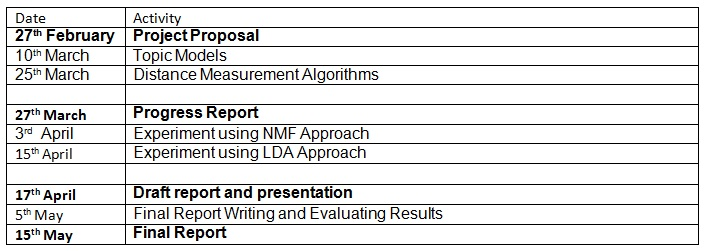
\includegraphics[scale=0.75]{schedule.jpg}
\end{figure}


\section{Budget}
\begin{figure}[h]
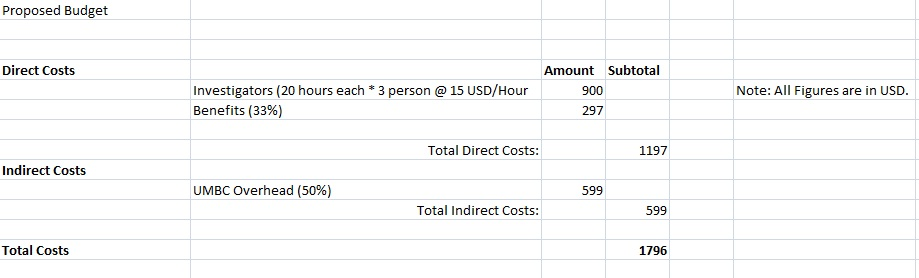
\includegraphics[scale=0.7]{Budget.jpg}
\end{figure}



\section{Appendix A: Research Conference}
The copy of the paper, 'Learning from Topic models - Going beyond SVD' by Sanjeev Arora, Rong Ge, Ankur Moitra from 53rd Annual IEEE Symposium on Foundations of Computer Science (FOCS 2012) research conference is attached.

\end{document}
